% Options for packages loaded elsewhere
\PassOptionsToPackage{unicode}{hyperref}
\PassOptionsToPackage{hyphens}{url}
\PassOptionsToPackage{dvipsnames,svgnames,x11names}{xcolor}
%
\documentclass[
  letterpaper,
  DIV=11,
  numbers=noendperiod]{scrartcl}

\usepackage{amsmath,amssymb}
\usepackage{iftex}
\ifPDFTeX
  \usepackage[T1]{fontenc}
  \usepackage[utf8]{inputenc}
  \usepackage{textcomp} % provide euro and other symbols
\else % if luatex or xetex
  \usepackage{unicode-math}
  \defaultfontfeatures{Scale=MatchLowercase}
  \defaultfontfeatures[\rmfamily]{Ligatures=TeX,Scale=1}
\fi
\usepackage{lmodern}
\ifPDFTeX\else  
    % xetex/luatex font selection
\fi
% Use upquote if available, for straight quotes in verbatim environments
\IfFileExists{upquote.sty}{\usepackage{upquote}}{}
\IfFileExists{microtype.sty}{% use microtype if available
  \usepackage[]{microtype}
  \UseMicrotypeSet[protrusion]{basicmath} % disable protrusion for tt fonts
}{}
\makeatletter
\@ifundefined{KOMAClassName}{% if non-KOMA class
  \IfFileExists{parskip.sty}{%
    \usepackage{parskip}
  }{% else
    \setlength{\parindent}{0pt}
    \setlength{\parskip}{6pt plus 2pt minus 1pt}}
}{% if KOMA class
  \KOMAoptions{parskip=half}}
\makeatother
\usepackage{xcolor}
\setlength{\emergencystretch}{3em} % prevent overfull lines
\setcounter{secnumdepth}{5}
% Make \paragraph and \subparagraph free-standing
\ifx\paragraph\undefined\else
  \let\oldparagraph\paragraph
  \renewcommand{\paragraph}[1]{\oldparagraph{#1}\mbox{}}
\fi
\ifx\subparagraph\undefined\else
  \let\oldsubparagraph\subparagraph
  \renewcommand{\subparagraph}[1]{\oldsubparagraph{#1}\mbox{}}
\fi


\providecommand{\tightlist}{%
  \setlength{\itemsep}{0pt}\setlength{\parskip}{0pt}}\usepackage{longtable,booktabs,array}
\usepackage{calc} % for calculating minipage widths
% Correct order of tables after \paragraph or \subparagraph
\usepackage{etoolbox}
\makeatletter
\patchcmd\longtable{\par}{\if@noskipsec\mbox{}\fi\par}{}{}
\makeatother
% Allow footnotes in longtable head/foot
\IfFileExists{footnotehyper.sty}{\usepackage{footnotehyper}}{\usepackage{footnote}}
\makesavenoteenv{longtable}
\usepackage{graphicx}
\makeatletter
\def\maxwidth{\ifdim\Gin@nat@width>\linewidth\linewidth\else\Gin@nat@width\fi}
\def\maxheight{\ifdim\Gin@nat@height>\textheight\textheight\else\Gin@nat@height\fi}
\makeatother
% Scale images if necessary, so that they will not overflow the page
% margins by default, and it is still possible to overwrite the defaults
% using explicit options in \includegraphics[width, height, ...]{}
\setkeys{Gin}{width=\maxwidth,height=\maxheight,keepaspectratio}
% Set default figure placement to htbp
\makeatletter
\def\fps@figure{htbp}
\makeatother

\KOMAoption{captions}{tableheading}
\makeatletter
\@ifpackageloaded{caption}{}{\usepackage{caption}}
\AtBeginDocument{%
\ifdefined\contentsname
  \renewcommand*\contentsname{Table of contents}
\else
  \newcommand\contentsname{Table of contents}
\fi
\ifdefined\listfigurename
  \renewcommand*\listfigurename{List of Figures}
\else
  \newcommand\listfigurename{List of Figures}
\fi
\ifdefined\listtablename
  \renewcommand*\listtablename{List of Tables}
\else
  \newcommand\listtablename{List of Tables}
\fi
\ifdefined\figurename
  \renewcommand*\figurename{Figure}
\else
  \newcommand\figurename{Figure}
\fi
\ifdefined\tablename
  \renewcommand*\tablename{Table}
\else
  \newcommand\tablename{Table}
\fi
}
\@ifpackageloaded{float}{}{\usepackage{float}}
\floatstyle{ruled}
\@ifundefined{c@chapter}{\newfloat{codelisting}{h}{lop}}{\newfloat{codelisting}{h}{lop}[chapter]}
\floatname{codelisting}{Listing}
\newcommand*\listoflistings{\listof{codelisting}{List of Listings}}
\makeatother
\makeatletter
\makeatother
\makeatletter
\@ifpackageloaded{caption}{}{\usepackage{caption}}
\@ifpackageloaded{subcaption}{}{\usepackage{subcaption}}
\makeatother
\ifLuaTeX
  \usepackage{selnolig}  % disable illegal ligatures
\fi
\usepackage{bookmark}

\IfFileExists{xurl.sty}{\usepackage{xurl}}{} % add URL line breaks if available
\urlstyle{same} % disable monospaced font for URLs
\hypersetup{
  pdftitle={AI Model Development for Urban Fabric Segmentation},
  pdfauthor={Barbara Metzler and Dani Arribas-Bel},
  colorlinks=true,
  linkcolor={blue},
  filecolor={Maroon},
  citecolor={Blue},
  urlcolor={Blue},
  pdfcreator={LaTeX via pandoc}}

\title{AI Model Development for Urban Fabric Segmentation}
\author{Barbara Metzler and Dani Arribas-Bel}
\date{}

\begin{document}
\maketitle

\renewcommand*\contentsname{Table of contents}
{
\hypersetup{linkcolor=}
\setcounter{tocdepth}{3}
\tableofcontents
}
This report includes the preliminary research and experiments run to
design an AI model for making predictions on the urban fabric of
England, as of November 2024.

\section{Executive Summary}\label{executive-summary}

This technical report details the development and evaluation of
artificial intelligence (AI) models for urban fabric classification and
segmentation using satellite imagery. The project spans from June 2024
to March 2025, encompassing model design, development, training, and
application to European urban strategy analysis. Our research compares
various approaches including classification and segmentation tasks,
using different foundation models as backbones. The primary goal is to
develop accurate and efficient methods for predicting urban fabric from
satellite imagery.

\section{Classification vs
segmentation}\label{classification-vs-segmentation}

In satellite image analysis, classification and segmentation address
spatial labeling at different levels of granularity, with classification
assigning a single label to an image tile or cell, while segmentation
provides pixel-level detail. In our study, the label dataset does not
always correspond directly to identifiable features in the imagery,
making classification a potentially more suitable approach as it
generalizes each tile's dominant land cover type without requiring exact
pixel alignment. However, we explore both approaches: classification for
broader pattern recognition and segmentation for finer,
boundary-specific mapping. This dual approach enables us to evaluate how
each method performs given the scale and feature alignment limitations
within the dataset.

\section{Methods}\label{methods}

\subsection{Data}\label{data}

\subsubsection{Satellite imagery (input)}\label{satellite-imagery-input}

The satellite image data used is accessed from the GHS-composite-S2
R2020A dataset \footnote{Corbane, C. et al., 2020. A global cloud-free
  pixel-based image composite from Sentinel-2 data. Data in brief, 31,
  p.105737.}. The dataset is a global, cloud-free image composite
derived from Sentinel-2 L1C data, covering the period from January 2017
to December 2018. We use three bands (RGB) and the images have a
resolution of 10 meters per pixel.

\subsubsection{Urban fabric classes
(outcome)}\label{urban-fabric-classes-outcome}

We use labels from the Spatial Signatures Framework \footnote{Fleischmann,
  M. \& Arribas-Bel, D., 2022. Geographical characterisation of British
  urban form using the spatial signatures framework. Scientific Data,
  9(1), p.546.}, which provides a typology of British urban environments
based on both form (physical appearance) and function (usage). Spatial
signatures capture complex urban characterizations, offering insights
into how different areas look and operate. While our primary interest is
in urban fabric classification focused on form---an approach we expect
may be simpler since form is visible in imagery---this classification
scheme is still under development. Therefore, we currently use the more
comprehensive Spatial Signatures Framework as a proxy, as it aligns with
the goals of urban characterization in our project.

\subsection{Data preprocessing}\label{data-preprocessing}

For our analysis, we use two datasets of image tiles at different
scales: larger tiles (224 x 224 pixels, covering 2240 x 2240 meters) for
segmentation tasks, and smaller tiles (56 x 56 pixels, covering 560 x
560 meters) for classification tasks. The segmentation dataset includes
26,753 tiles (21,402 for training and 5,351 for testing), while the
classification dataset consists of 403,722 tiles (342,648 for training
and 61,074 for testing). For consistent sampling and comparison, we only
use tiles that fully overlap with the spatial signatures, ensuring that
each tile aligns with the urban form and function typology in our
labeling framework. This alignment supports robust comparison of
classification and segmentation outcomes on a pixel-level.

\begin{center}
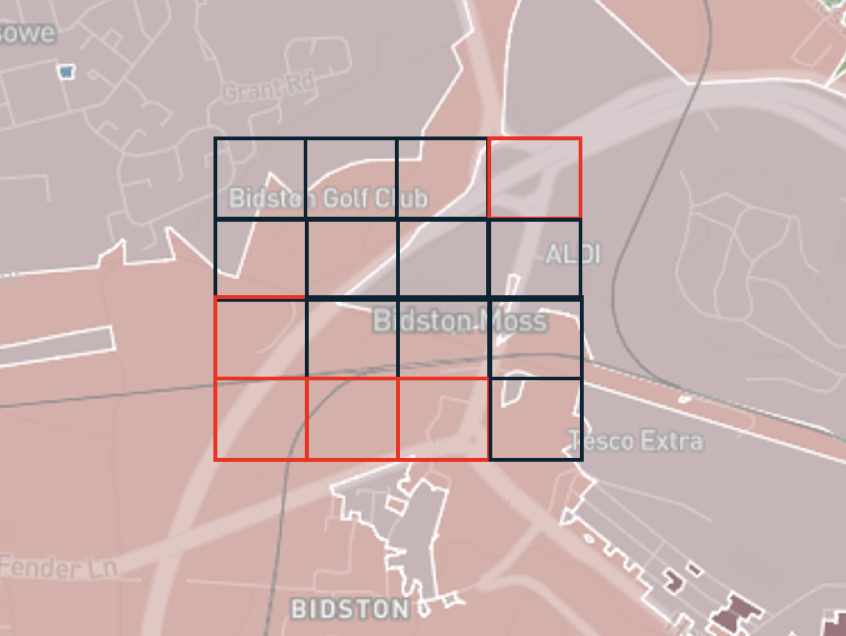
\includegraphics[width=\textwidth,height=4.16667in]{../figures/algo_design/sampling.png}
\end{center}

A significant challenge in our dataset is class imbalance, where certain
urban fabric types are substantially more represented than others. This
imbalance influenced our decisions regarding model architecture and loss
function selection, leading us to explore specialized approaches for
handling uneven class distributions.

\subsubsection{Train/test split}\label{traintest-split}

We split the dataset into 80\% train and 20\% test data. The test
datasets for segmentation and classification overlap.

\begin{center}
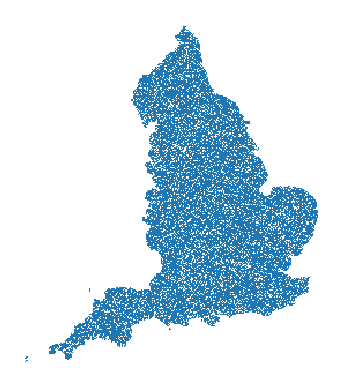
\includegraphics[width=\textwidth,height=4.16667in]{../figures/algo_design/train_df.png}
\end{center}
\begin{center}
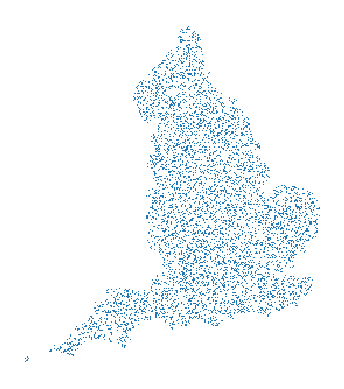
\includegraphics[width=\textwidth,height=4.16667in]{../figures/algo_design/test_df.png}
\end{center}

\subsubsection{Unbalanced dataset}\label{unbalanced-dataset}

\begin{center}
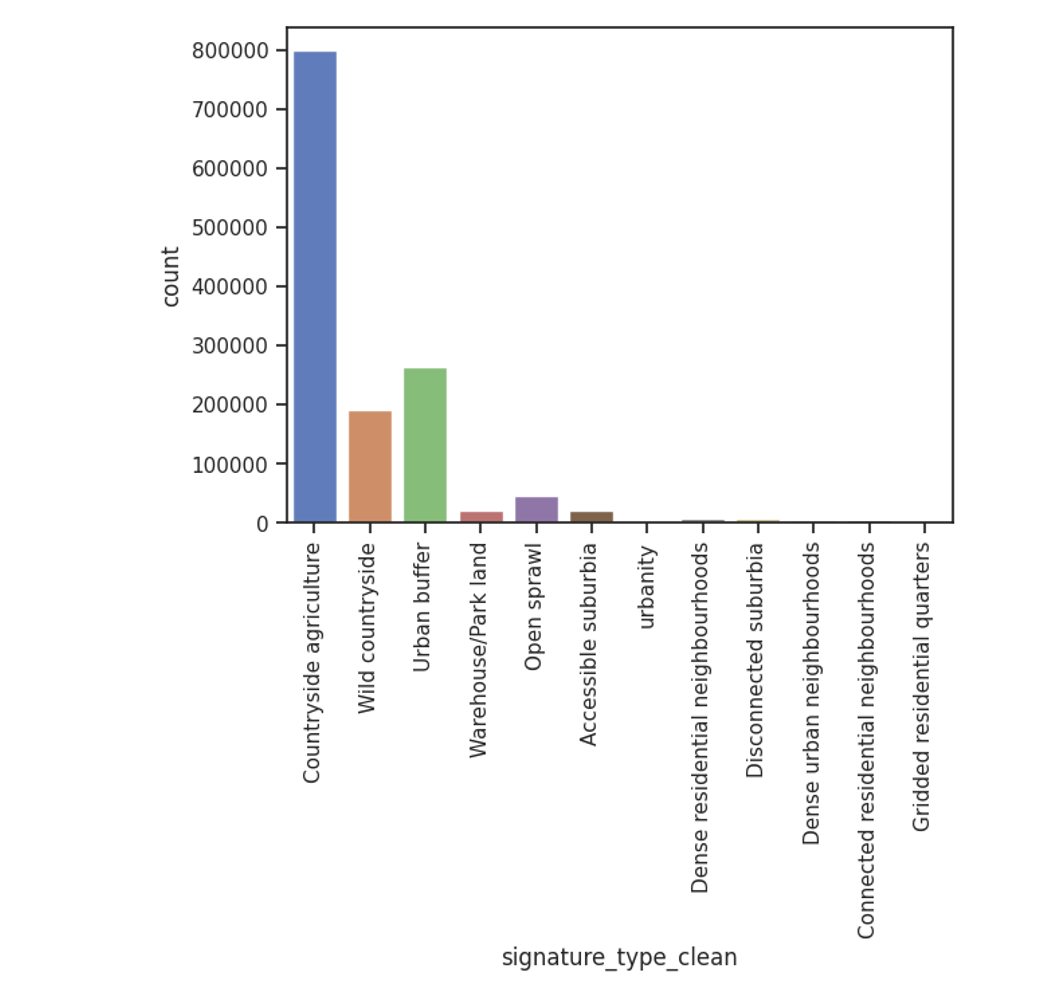
\includegraphics[width=\textwidth,height=4.375in]{../figures/algo_design/unbalanced.png}
\end{center}

\section{Model architectures}\label{model-architectures}

Our study involves three main experiments to analyze urban fabric
classification and segmentation. First, we conduct a baseline experiment
using image embeddings from the SatlasPretrain model \footnote{Bastani,
  F. et al., 2023. Satlaspretrain: A large-scale dataset for remote
  sensing image understanding. In Proceedings of the IEEE/CVF
  International Conference on Computer Vision, pp.~16772-16782.}, which
we fit to an XGBoost classifier to predict urban fabric classes
(Approach A). Second, we fine-tune three different geospatial foundation
models---SatlasPretrain, Clay, and IBM/NASA's Prithvi model---to perform
segmentation tasks (Approach B). Third, we take the best-performing
geospatial foundation model from the segmentation experiments (Clay) and
fine-tune it specifically for a classification task (Approach C). To
evaluate and compare the results, we report weighted pixel-level
accuracy, F1 score, and Intersection over Union (IoU) metrics across the
experiments.

\begin{itemize}
\tightlist
\item
  Approach A: Image embeddings + XGBoost model
\item
  Approach B: Fine-tuned geospatial foundation model (segmentation)
\item
  Approach C: Fine-tuned geospatial foundation model (classification)
\end{itemize}

\subsection{Baseline approach (Approach
A)}\label{baseline-approach-approach-a}

The tiles are fed into the geospatial foundation model SatlasPretrain
\footnote{Bastani, F. et al., 2023. Satlaspretrain: A large-scale
  dataset for remote sensing image understanding. In Proceedings of the
  IEEE/CVF International Conference on Computer Vision, pp.~16772-16782.}
that has been pretrained with more than 302 million labels on a range of
remote sensing and computer vision tasks.

The model operates in two main steps:

\begin{enumerate}
\def\labelenumi{\arabic{enumi}.}
\tightlist
\item
  Foundation Model: A vision transformer model with a feature pyramid
  network (FPN) and a pooling layer is used to derive image
  embeddings---lower-dimensional representations of the images (Fig. 2).
\item
  Machine Learning Classifier: The image embeddings are then input into
  an XGBoost classifier to predict urban fabric classes across England.
\end{enumerate}

Our baseline model achieved a moderate prediction accuracy of
approximately 61\% with varying accuracy across the various spatial
signature classes as seen in the figure below.

\begin{center}
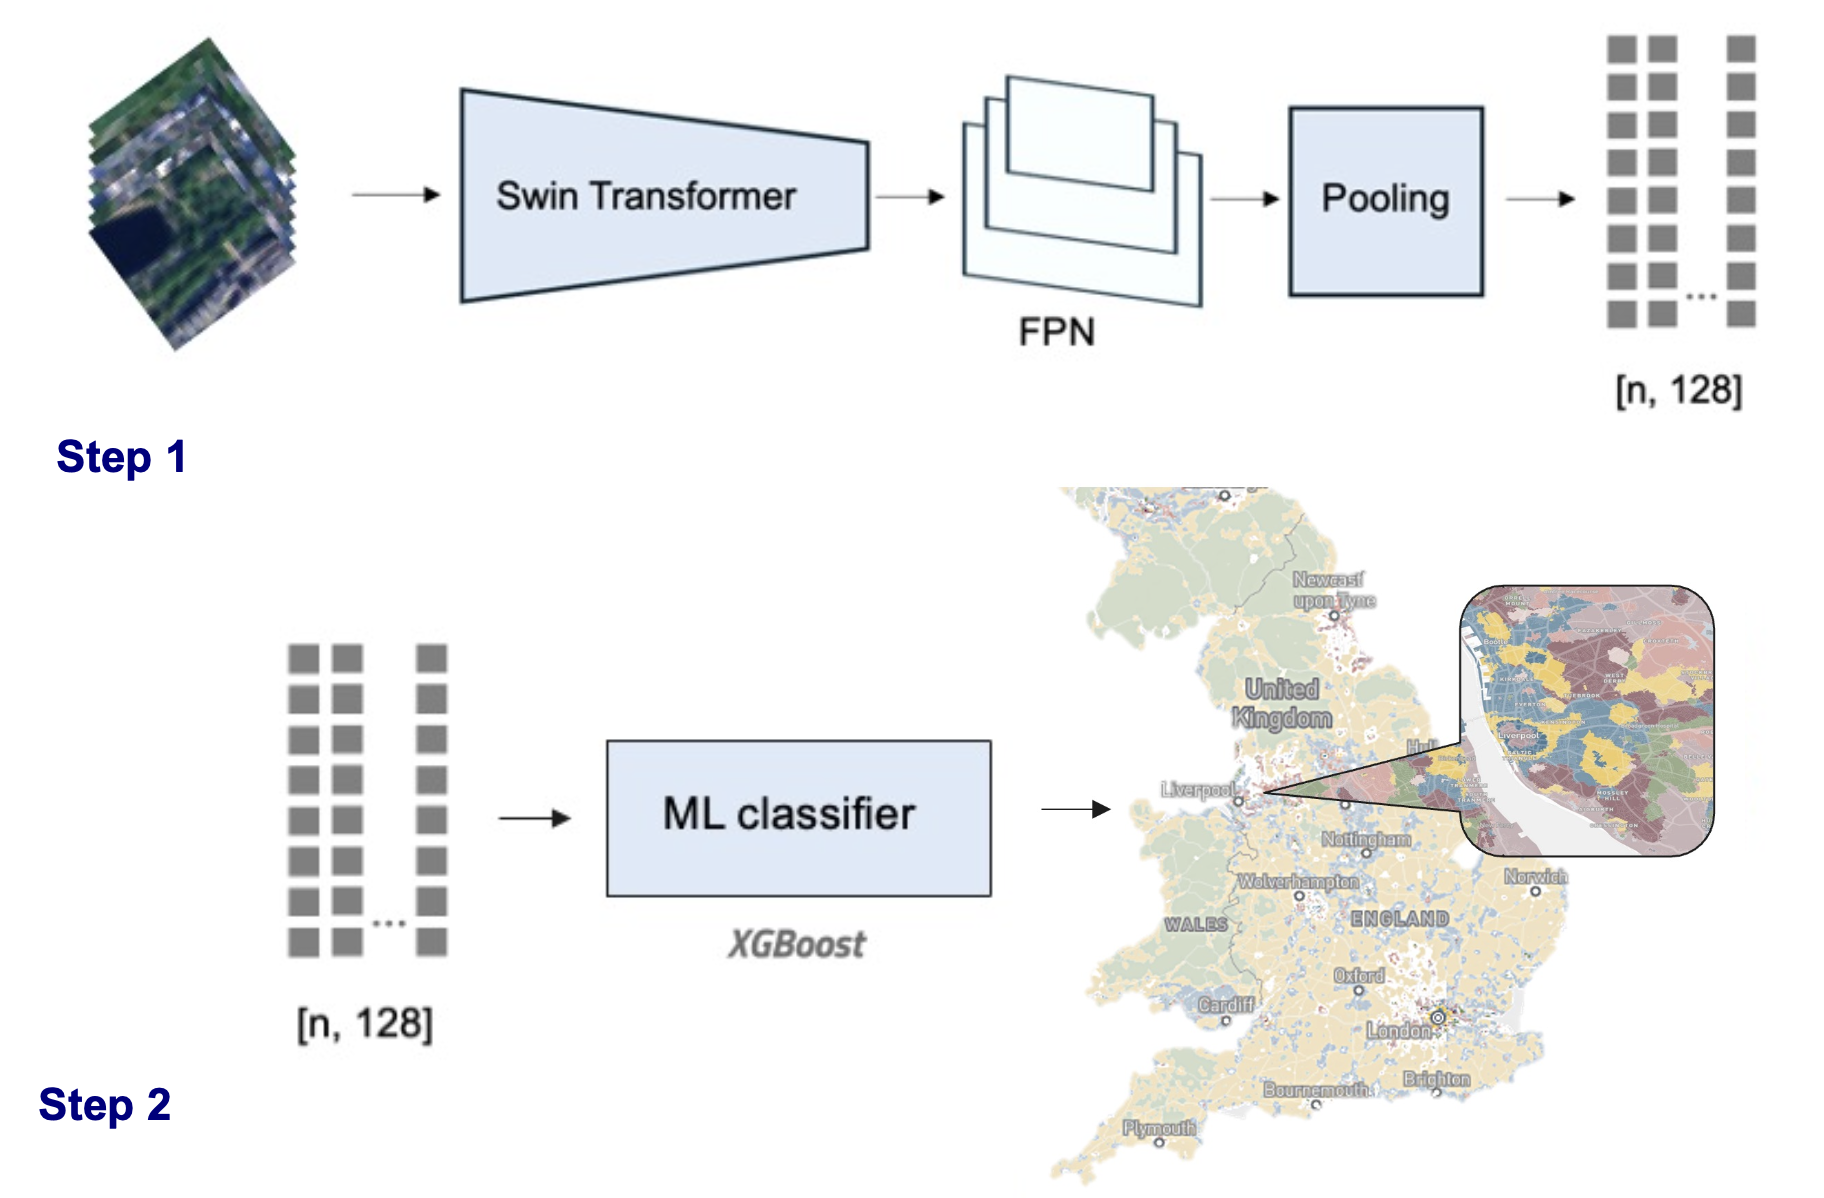
\includegraphics[width=\textwidth,height=4.16667in]{../figures/algo_design/baseline.png}
\end{center}

\subsubsection{Results across spatial
signatures}\label{results-across-spatial-signatures}

\begin{center}
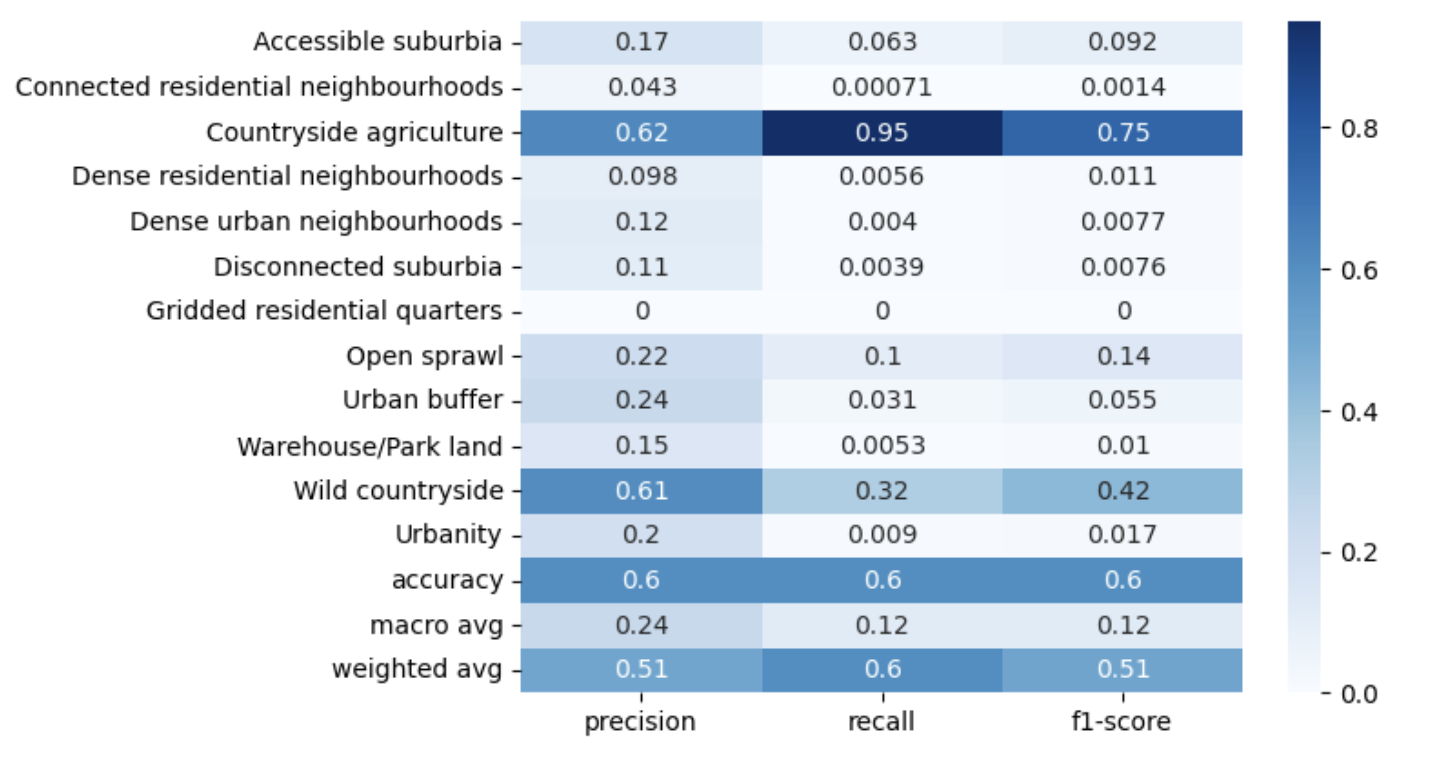
\includegraphics[width=\textwidth,height=4.375in]{../figures/algo_design/baseline_tile_level.png}
\end{center}

\emph{Baseline approach (ordinal)}

In addition to the general classification task, we explored an ordinal
regression task to account for the continuous nature of the spatial
signatures, which are not strictly categorical. We applied the following
ordinal mapping:

\texttt{ordinal\_mapping\ =\ \{\ \ \ \ \ \textquotesingle{}Wild\ countryside\textquotesingle{}:\ 0,\ \ \ \ \ \textquotesingle{}Countryside\ agriculture\textquotesingle{}:\ 1,\ \ \ \ \ \textquotesingle{}Urban\ buffer\textquotesingle{}:\ 2,\ \ \ \ \ \textquotesingle{}Open\ sprawl\textquotesingle{}:\ 3,\ \ \ \ \ \textquotesingle{}Disconnected\ suburbia\textquotesingle{}:\ 4,\ \ \ \ \ \textquotesingle{}Accessible\ suburbia\textquotesingle{}:\ 5,\ \ \ \ \ \textquotesingle{}Warehouse/Park\ land\textquotesingle{}:\ 6,\ \ \ \ \ \textquotesingle{}Gridded\ residential\ quarters\textquotesingle{}:\ 7,\ \ \ \ \ \textquotesingle{}Connected\ residential\ neighbourhoods\textquotesingle{}:\ 8,\ \ \ \ \ \textquotesingle{}Dense\ residential\ neighbourhoods\textquotesingle{}:\ 9,\ \ \ \ \ \textquotesingle{}Dense\ urban\ neighbourhoods\textquotesingle{}:\ 10,\ \ \ \ \ \textquotesingle{}Urbanity\textquotesingle{}:\ 11,\ \}}

This ordinal approach produced a Mean Absolute Error (MAE) and Mean
Squared Error (MSE) of 0.28, along with an R² score of 0.62. The Sankey
diagram below highlights the primary misclassifications, which tend to
occur between similar classes.

\begin{center}
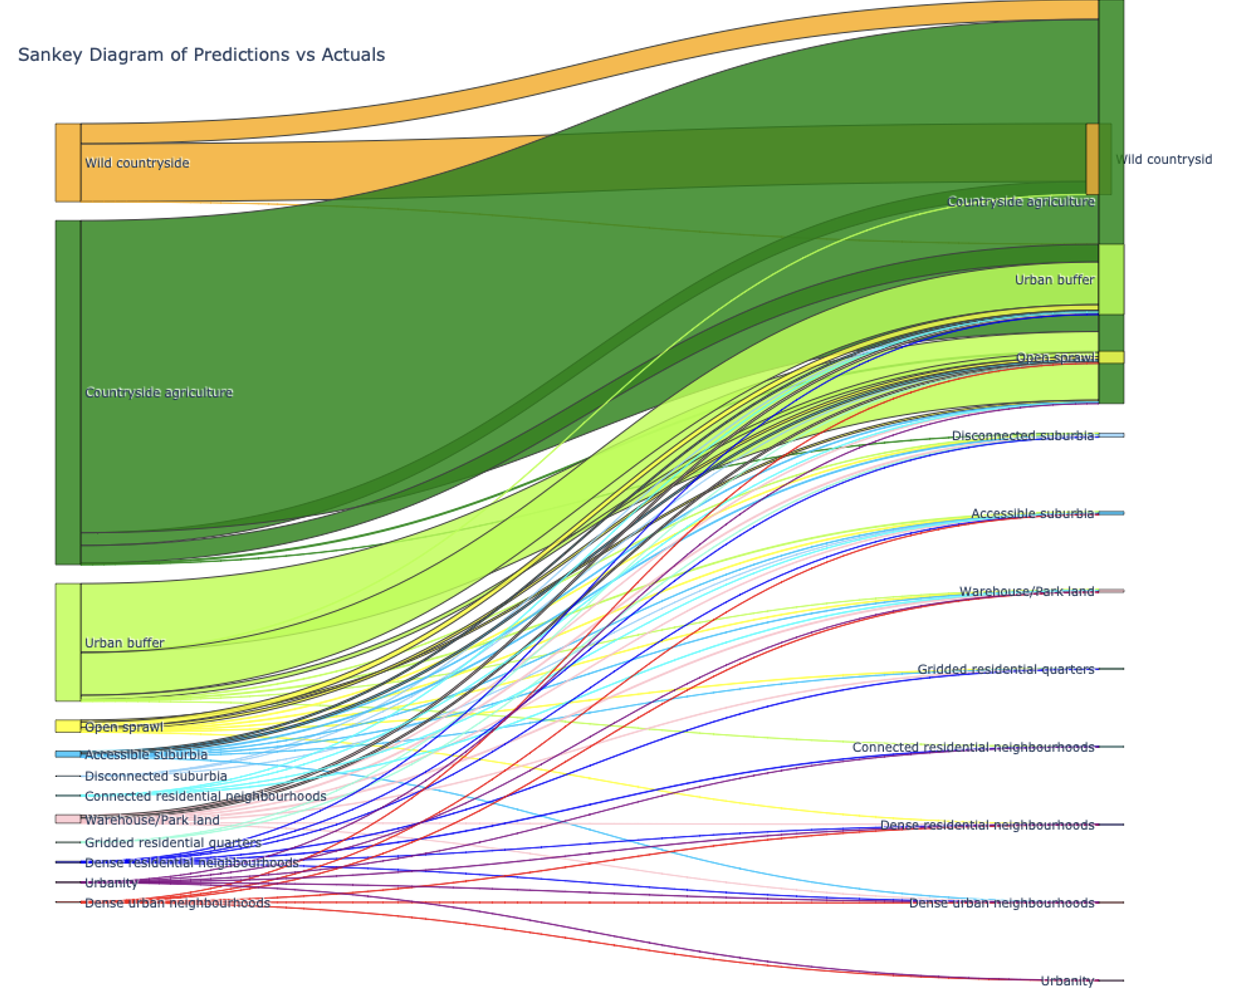
\includegraphics[width=\textwidth,height=4.375in]{../figures/algo_design/sankey.png}
\end{center}

\emph{Baseline approach + spatial context}

To enhance model performance, we incorporated spatial context, enabling
the model to account for regional location. We included H3 Level 5
hexagon identifiers as a categorical variable, where each hexagon
(approximately 560x560 meters) encompasses around 80 tiles.

\begin{center}
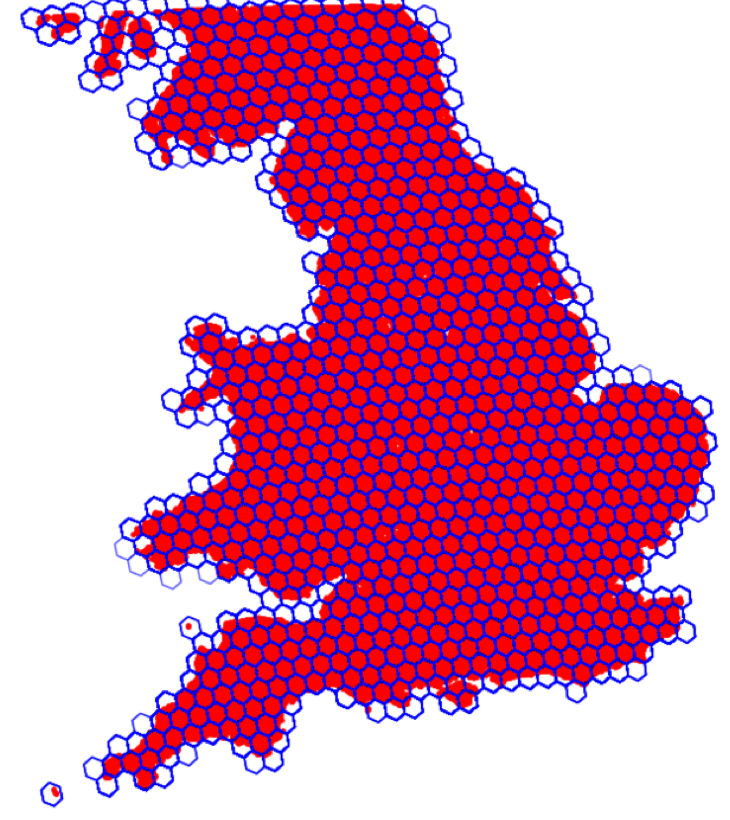
\includegraphics[width=\textwidth,height=4.375in]{../figures/algo_design/hex_level5.png}
\end{center}

\subsection{Segmentation (Approach B)}\label{segmentation-approach-b}

In Approach B, we fine-tuned a state-of-the-art geospatial foundation
model for a segmentation task. We used the 224x224x3 image tiles as
input. We evaluated three state-of-the-art foundation models, each with
unique characteristics as listed below:

\begin{longtable}[]{@{}llll@{}}
\toprule\noalign{}
Model & Architecture & Dataset Size & Image Sources \\
\midrule\noalign{}
\endhead
\bottomrule\noalign{}
\endlastfoot
Satlas \footnote{Corbane, C. et al., 2020. A global cloud-free
  pixel-based image composite from Sentinel-2 data. Data in brief, 31,
  p.105737.} & SwinT & 302M labels & Sentinel-2 \\
Clay \footnote{https://huggingface.co/made-with-clay/Clay} & MAE/ViT &
70M labels & Multiple+ \\
Prithvi \footnote{https://huggingface.co/ibm-nasa-geospatial/Prithvi-100M}
& MAE/ViT & 250 PB & Sentinel-2/Landsat \\
\end{longtable}

+Multiple sources include Sentinel-2, Landsat, NAIP, and LINZ

The following visualisations show the varying model configurations for
the three different approaches tested for the segmentation task. The
main difference is the varying backbone.

\subsubsection{Model A: Satlas}\label{model-a-satlas}

\begin{center}
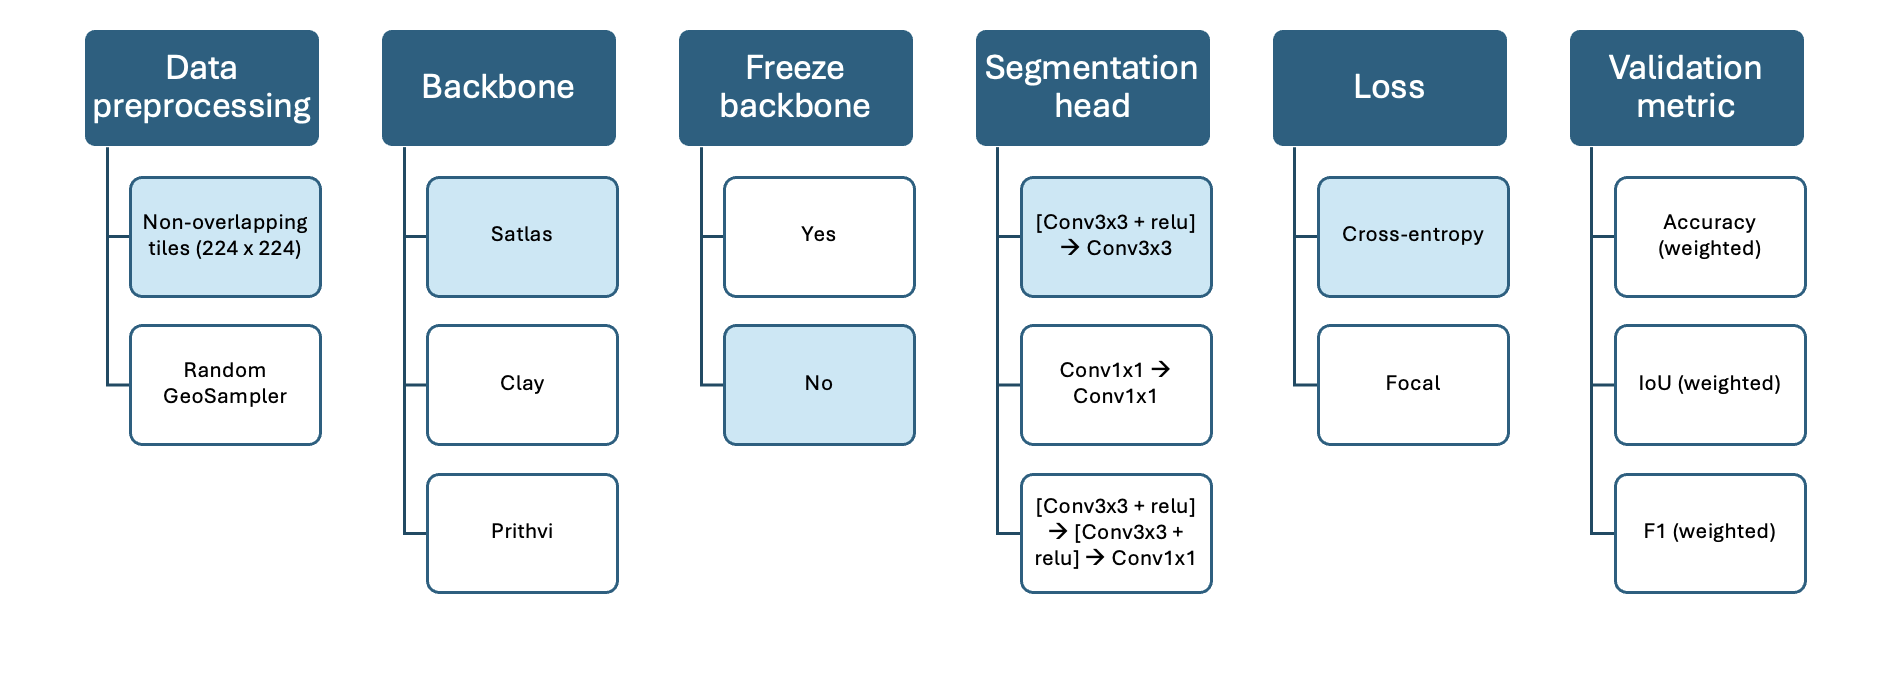
\includegraphics[width=6.25in,height=\textheight]{../figures/algo_design/satlas_model.png}
\end{center}

\begin{center}\rule{0.5\linewidth}{0.5pt}\end{center}

\subsubsection{Model B: Clay}\label{model-b-clay}

\begin{center}
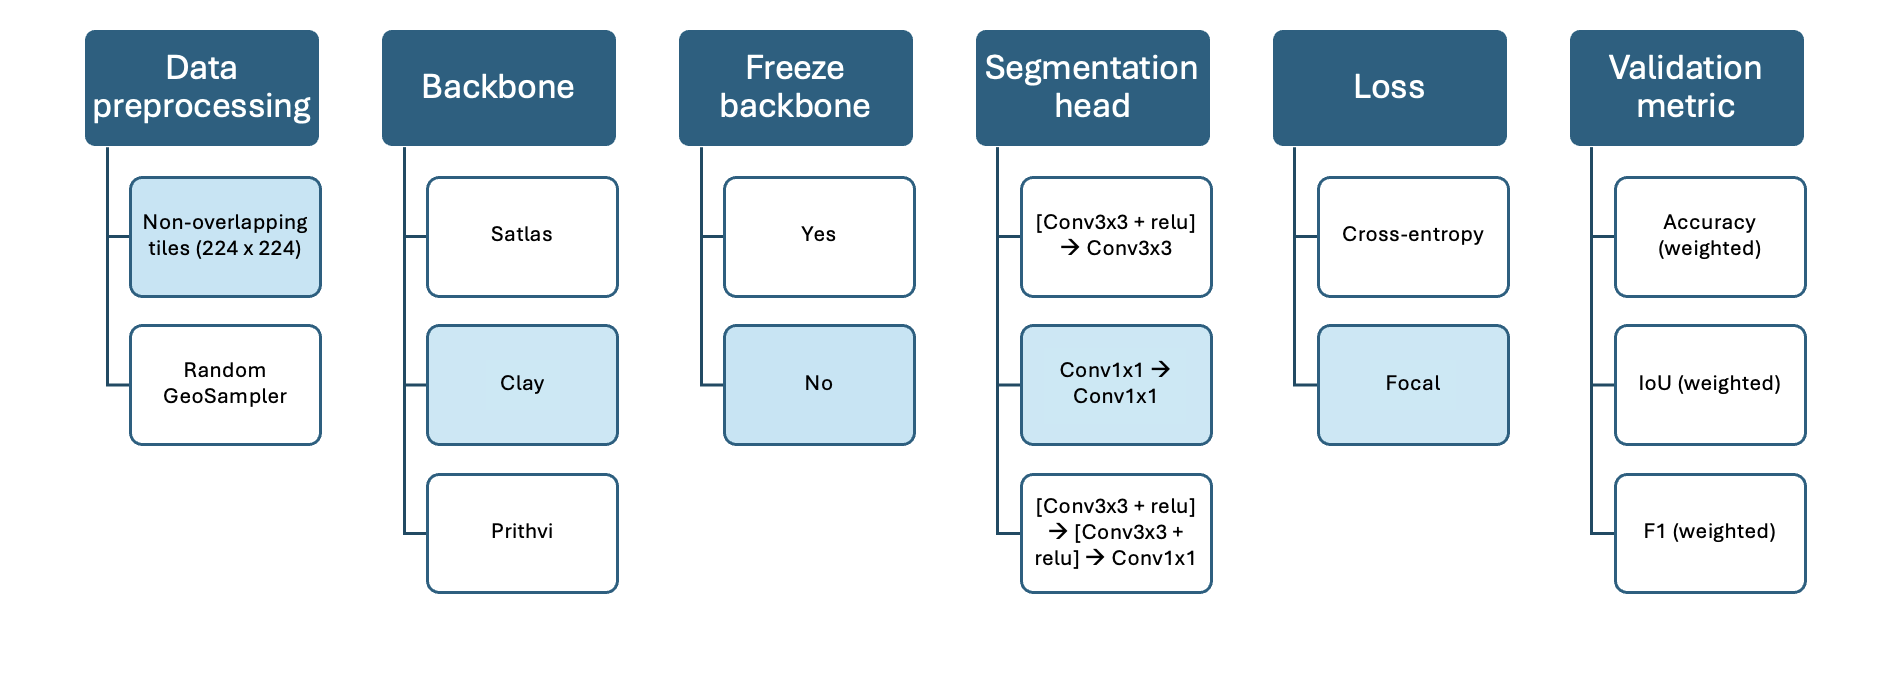
\includegraphics[width=6.25in,height=\textheight]{../figures/algo_design/clay_model.png}
\end{center}

\begin{center}\rule{0.5\linewidth}{0.5pt}\end{center}

\subsubsection{Model C: Prithvi}\label{model-c-prithvi}

\begin{center}
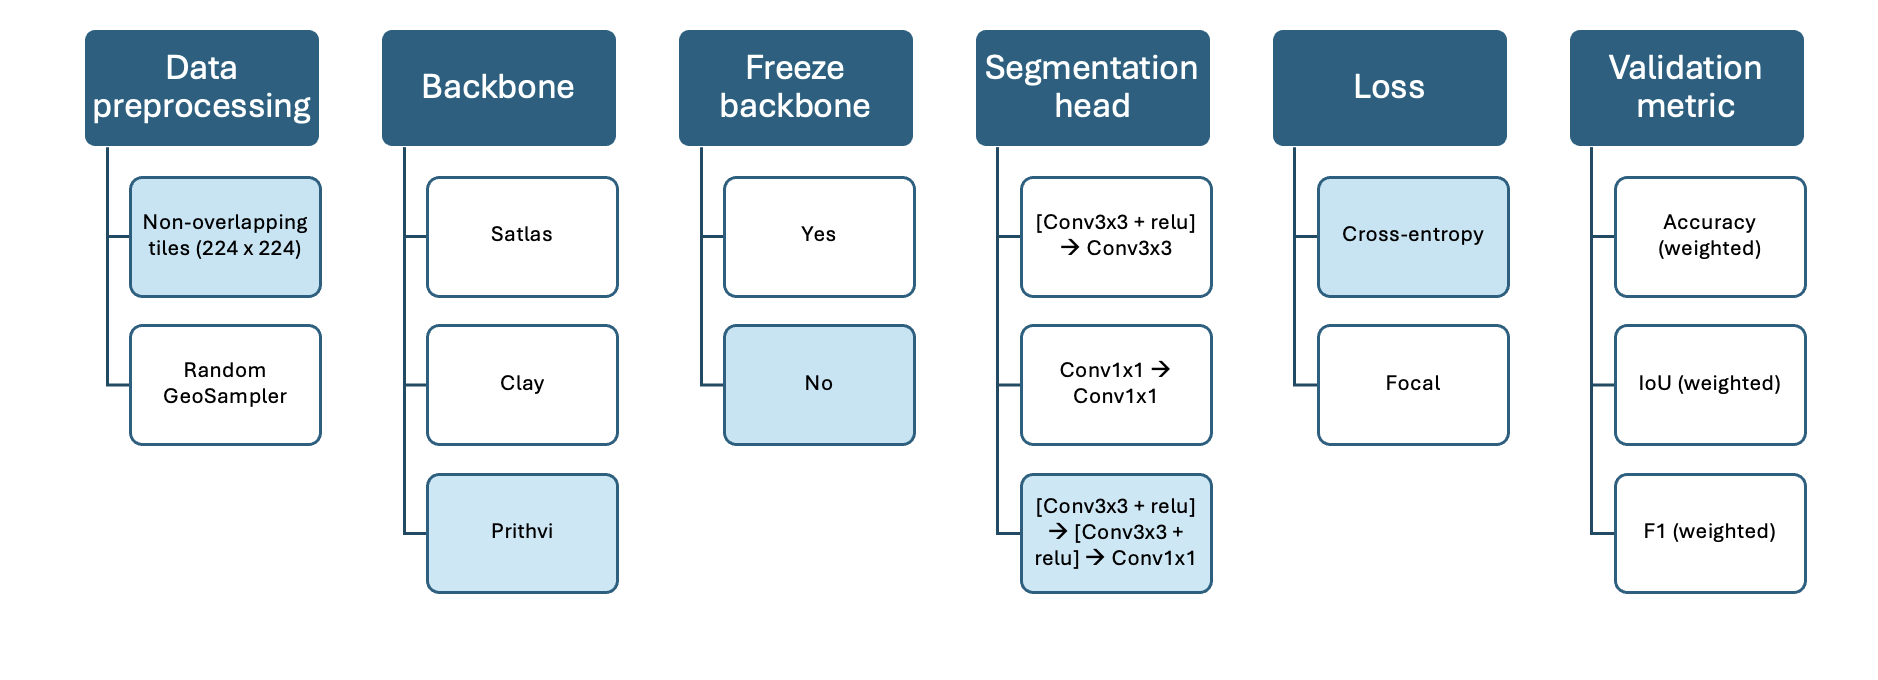
\includegraphics[width=6.25in,height=\textheight]{../figures/algo_design/prithvi_model.png}
\end{center}

After fine-tuning each foundation model for 10 epochs, we observed the
following performance metrics:

\begin{longtable}[]{@{}llll@{}}
\toprule\noalign{}
Metric & Satlas & Clay & Prithvi \\
\midrule\noalign{}
\endhead
\bottomrule\noalign{}
\endlastfoot
Weighted Accuracy & 0.57 & \textbf{0.72} & 0.62 \\
Weighted IoU & 0.33 & \textbf{0.58} & 0.41 \\
Weighted F1 & 0.41 & \textbf{0.69} & 0.58 \\
Training Time/Epoch & 9 mins & 8 mins & 20 mins \\
Parameters & 90M & 86M & 120M \\
Implementation Score & 5/10 & 6/10 & 7/10 \\
\end{longtable}

The Clay model consistently outperformed other foundation models across
all metrics, while also maintaining reasonable training times and
computational requirements.

\textbf{Loss Function Impact:} The choice of loss function significantly
influenced model performance. Focal loss proved particularly effective
in handling class imbalance, especially when combined with the Clay
model architecture.

\subsection{Classification (Approach
C)}\label{classification-approach-c}

Finally, in Approach C, we fine-tuned a geospatial foundation model for
a classification task. We used the 56x56x3 image tiles as input.

For this approach we only used the Clay model as backbone, since it
performed the best in the previous experiments.

The accuracy varied across the different classes as seen in the figure
below:

\begin{center}
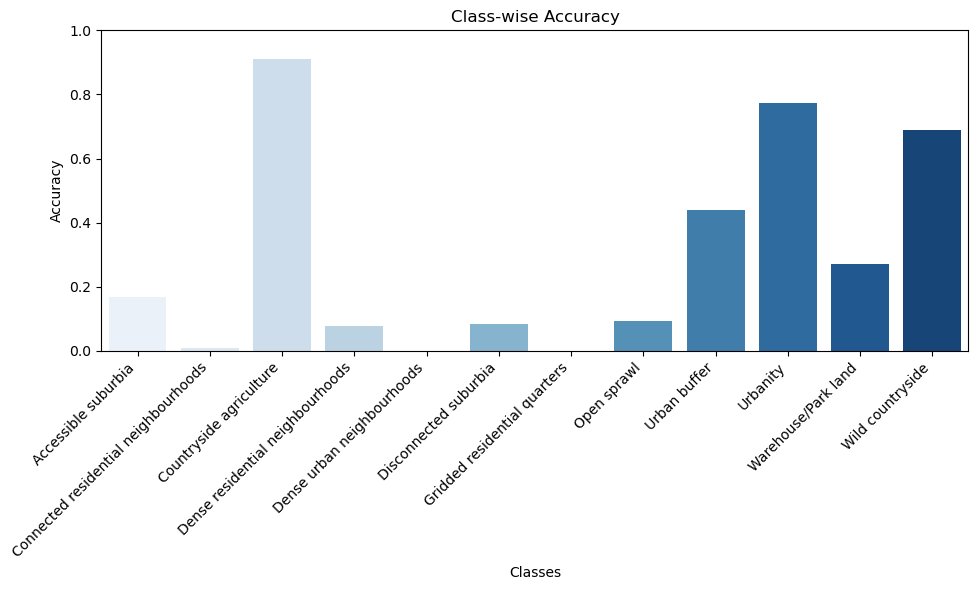
\includegraphics[width=\textwidth,height=4.47917in]{../figures/algo_design/class_acc.png}
\end{center}

This figure shows a comparison between the predicted classes for the
fine-tuned geospatial foundation model with segmentation approach (B)
and the classification (C).

\begin{center}
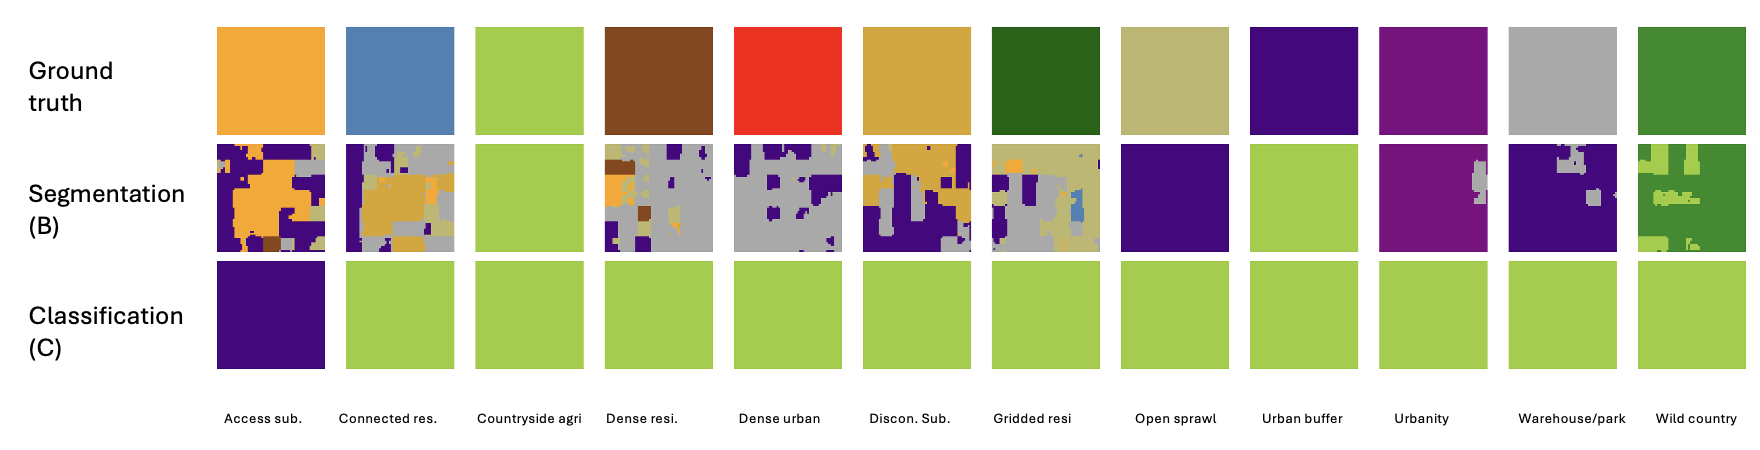
\includegraphics[width=\textwidth,height=4.47917in]{../figures/algo_design/comparison_B_C.png}
\end{center}

\subsubsection{Evaluation Metrics}\label{evaluation-metrics}

We employed multiple complementary metrics to evaluate model
performance, as follows:

\begin{enumerate}
\def\labelenumi{\arabic{enumi}.}
\item
  \textbf{Intersection over Union (IoU):} This metric measures the
  overlap between predicted and ground truth segmentations, ranging from
  0 (no overlap) to 1 (perfect overlap). IoU is calculated as the area
  of intersection divided by the area of union between the predicted and
  actual segmentation masks.
\item
  \textbf{Weighted F1 Score:} This metric provides a balanced measure of
  precision and recall, particularly important for imbalanced datasets.
  It is calculated as the harmonic mean of precision (how many of the
  predicted positives are correct) and recall (how many of the actual
  positives were identified), weighted by class frequencies.
\item
  \textbf{Weighted Accuracy:} This metric calculates the proportion of
  correct predictions, weighted by class frequencies to account for
  class imbalance. It provides a more representative measure of model
  performance across all classes, regardless of their frequency in the
  dataset.
\end{enumerate}

\section{Results}\label{results}

Comparing the results is a non-trivial task because the image tiles do
not correspond to each other and do not perfectly overlap (42px vs 224
px). To make a fair comparison we thus calculate the pixel-level
accuracy scores across the approaches. For this purpose, we predict the
full map of the test set and compare the overlapping tiles (as described
in sampling). We then calculate the following metrics on a per-pixel
level.

\subsection{Overall model performance comparison
(Pixel-level)}\label{overall-model-performance-comparison-pixel-level}

Our comprehensive evaluation revealed varying levels of performance
across the three different approaches:

\begin{longtable}[]{@{}
  >{\raggedright\arraybackslash}p{(\columnwidth - 8\tabcolsep) * \real{0.1754}}
  >{\raggedright\arraybackslash}p{(\columnwidth - 8\tabcolsep) * \real{0.2807}}
  >{\raggedright\arraybackslash}p{(\columnwidth - 8\tabcolsep) * \real{0.2807}}
  >{\raggedright\arraybackslash}p{(\columnwidth - 8\tabcolsep) * \real{0.1754}}
  >{\raggedright\arraybackslash}p{(\columnwidth - 8\tabcolsep) * \real{0.0877}}@{}}
\toprule\noalign{}
\begin{minipage}[b]{\linewidth}\raggedright
Approach
\end{minipage} & \begin{minipage}[b]{\linewidth}\raggedright
Global Accuracy
\end{minipage} & \begin{minipage}[b]{\linewidth}\raggedright
Macro Accuracy
\end{minipage} & \begin{minipage}[b]{\linewidth}\raggedright
F1 Score
\end{minipage} & \begin{minipage}[b]{\linewidth}\raggedright
IoU
\end{minipage} \\
\midrule\noalign{}
\endhead
\bottomrule\noalign{}
\endlastfoot
Classification (embeddings) & 0.76 (0.66) & 0.22 (0.13) & 0.23 & 0.63 \\
Classification + H3 level 5 & \textbf{0.87} (0.82) & \textbf{0.42}
(0.35) & \textbf{0.45} & \textbf{0.79} \\
Classification + H3 ordinal & 0.80 (0.80) & 0.26 (0.26) & 0.26 & 0.69 \\
Classification (Clay) & 0.59 (0.68) & 0.09 & 0.12 & 0.38 \\
Segmentation (Clay) & 0.73 & 0.31 & 0.30 & 0.58 \\
\end{longtable}

The baseline classification approaches demonstrated varying levels of
success: - Basic embedding classification achieved 76\% global accuracy
(66\% balanced) - Integration with H3 level 5 spatial indexing
significantly improved performance to 87\% global accuracy (42\%
balanced) - H3 level 5 ordinal classification reached 80\% accuracy
(26\% balanced)

The fine-tuned geospatial foundation model performed better than the
fine-tuned classification, with an accuracy score of 0.56 and 0.73
respectively.

Overall, the baseline approach with regional information performed best.
This approach is not only the best performing but also relatively
efficient to implement. Once the image embeddings are created, the
downstream classification can be done in minutes.

\subsubsection{Prediction example:
London}\label{prediction-example-london}

The following figure shows an example of a prediction for the London
area using the whole dataset. Each colour represents a different
signature. The background colour represents the ground truth.

\begin{center}
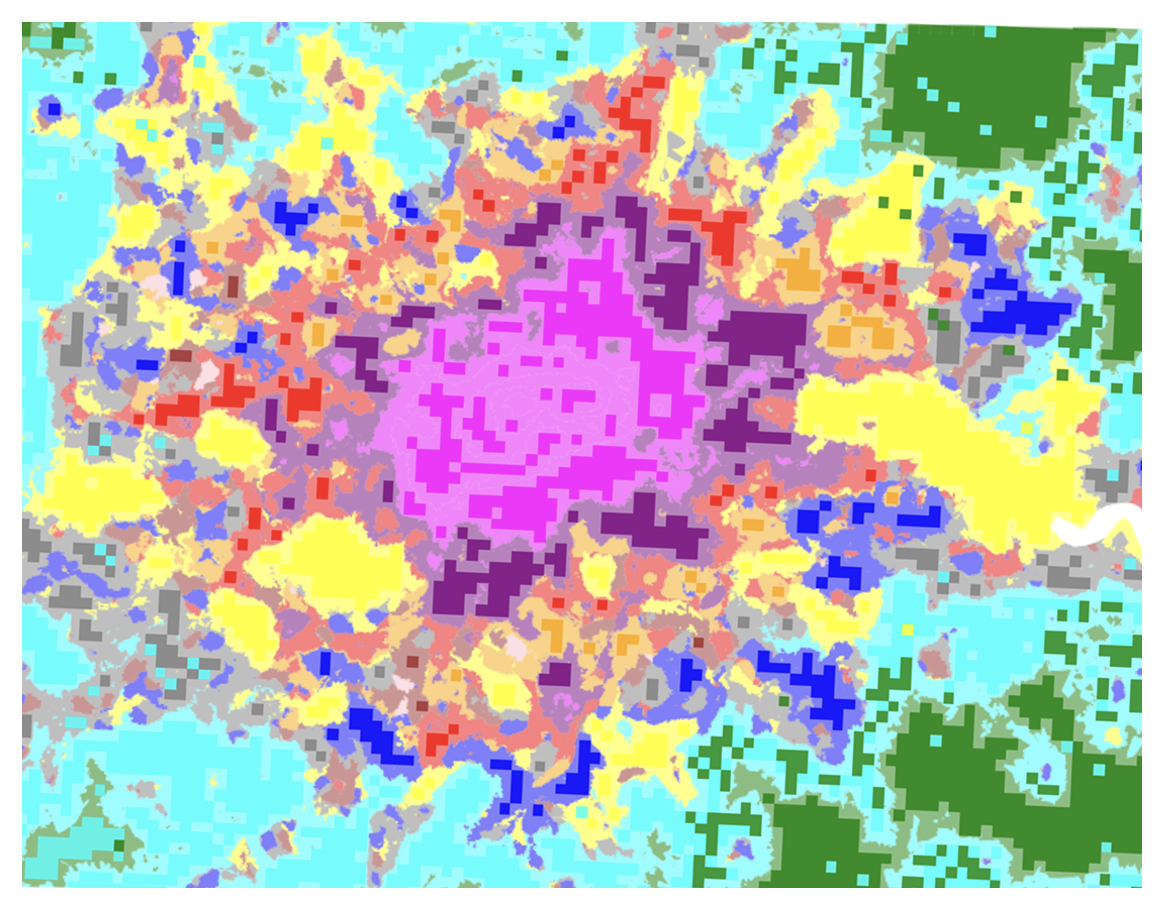
\includegraphics[width=\textwidth,height=4.375in]{../figures/algo_design/results_eurofab.png}
\end{center}

\section{Discussion}\label{discussion}

\subsubsection{Spatial signatures: Example
tiles}\label{spatial-signatures-example-tiles}

\begin{center}
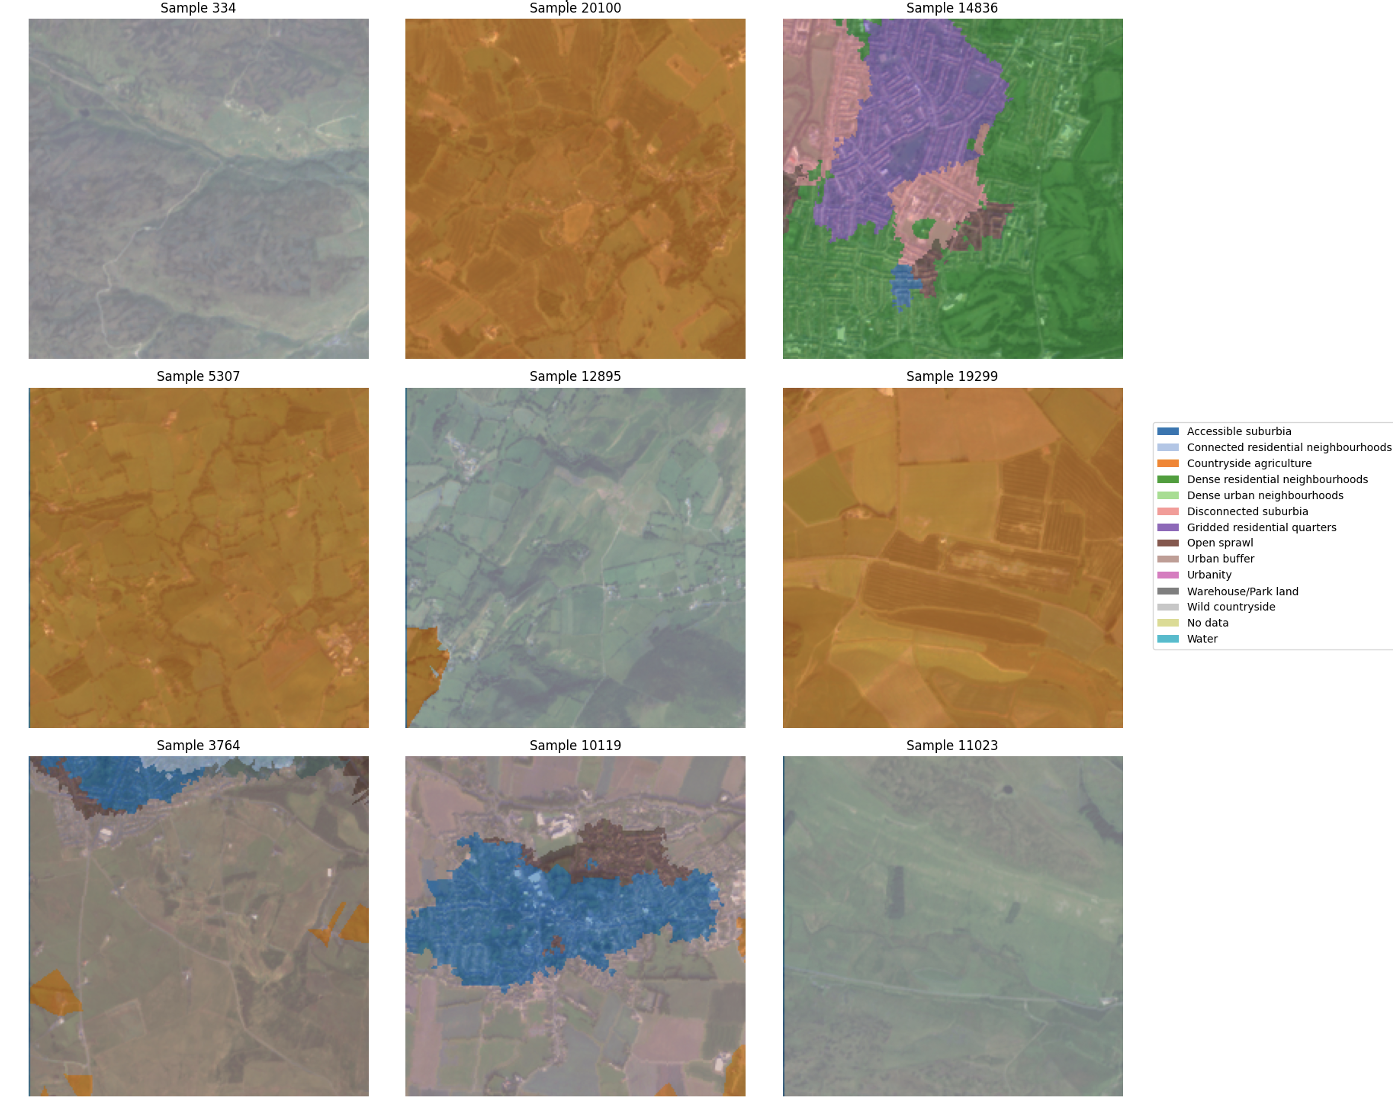
\includegraphics[width=\textwidth,height=4.375in]{../figures/algo_design/random_sample.png}
\end{center}

\subsection{Key Findings}\label{key-findings}

\begin{enumerate}
\def\labelenumi{\arabic{enumi}.}
\item
  \textbf{Regional trends:} The integration of regional information into
  the model significantly improving model performance across all
  metrics.
\item
  \textbf{Model performance:}:
\end{enumerate}

\subsection{Challenges and
Limitations}\label{challenges-and-limitations}

Our research encountered several significant challenges:

\begin{enumerate}
\def\labelenumi{\arabic{enumi}.}
\item
  \textbf{Class Imbalance:} The dataset exhibited substantial variations
  in class representation, which impacted model performance. While focal
  loss helped address this issue, some classes remained challenging to
  predict accurately.
\item
  \textbf{Computational Resources:} Training times varied significantly
  between models, with Prithvi requiring substantially more
  computational resources. This presents practical considerations for
  model deployment and scaling.
\item
  \textbf{Comparison Complexity:} The different tile sizes between
  classification (42px) and segmentation (224px) approaches made direct
  comparisons challenging, requiring careful consideration of evaluation
  metrics and methodology.
\end{enumerate}

\section{Conclusions}\label{conclusions}

Our research demonstrates that combining classification with
hierarchical spatial structuring (H3) provides the most effective
approach for urban fabric segmentation. While foundation models show
promise, their effectiveness varies significantly, with Clay emerging as
the most suitable backbone for our specific use case. The use of
appropriate loss functions, particularly focal loss, proves crucial in
handling dataset imbalances. These findings provide a solid foundation
for future development of urban fabric analysis tools and methodologies.



\end{document}
